\documentclass[12pt, letter]{article}

%% Class name and Assignment number
%%
\newcommand{\courseName}{Introduction~to~Deep~Learning~for~Computer~Vision}
\newcommand{\assignName}{Assignment~3:~Simple~Linear~Classifier II}

%% Packages
\usepackage{amsmath,amsfonts,amssymb,amsthm,dsfont}
\usepackage{graphicx}
\usepackage[bookmarks=false]{hyperref}
\usepackage{color}
\usepackage{lipsum}

%% Paper format
\usepackage{geometry}
\geometry{
    letterpaper,
    %% total={216mm,279mm}, %< NSERC size
    margin=2.00cm,     %< default
    %% margin=1.87cm,       %< NSERC tightest
}

%% Headers and footers
\usepackage[explicit]{titlesec}
\newpagestyle{titlesec_assignment}{
  \sethead{\courseName}{}{\assignName}\setfoot{}{\thepage}{}
  \headrule
  %% \footrule
}

\usepackage{graphicx}
\graphicspath{ {./images/} }

\begin{document}

%% Set header and footer
\pagestyle{titlesec_assignment}

%% Title
\title{\courseName\\\assignName}
\author{Paul Molina-Plant}
\maketitle

\abstract{In this assignment, I finished a implementing a linear classifier.
  This included implementing the loss function for logistic regression and
  implementing cross validation. \\

  In section 1, I derive the gradient for cross entropy use in logistic
  regression. \\
  The weights gradient is,
  \begin{equation}\nonumber\frac{\partial L_i}{\partial W} = (P_{ij} -
    \delta_{ij}) x_i \end{equation}
  And the bias gradient is,
  \begin{equation}\nonumber\frac{\partial L_i}{\partial b_i} = P_{ij} -
    \delta_{ij}\end{equation}

  In section 2, I plotted the results of the classifier being run on cifar10 in linear svm and
  logistic regression mode. For this dataset, linear svm produced a marginally more
  accurate model. \\

  In section 3, I plotted the results of the classifier being run in logistic
  regression mode with cross validation. I ran the classifer twice, once with a
  learning rate of $lr_1 = 10^{-4}$ and then with $lr_2 = 10^{-2}$. I observed
  that the accuracy and loss plots of $lr_1$ stabalize quickly, which means
  $lr_1$ is a good learning rate. In contrast, the plots of $lr_2$ never
  stabilizes because the learning rate is too high, causing the descent algorithm
  to consistently overshoot.

\pagebreak

\section{Derivation of the gradient for cross entropy}
\subsection{The cross entropy function}
\begin{equation}
  L_i = - log \frac{\sum_jt_{ij}e^{s_{ij}}}{\sum_ke^{s_{ik}}}
\end{equation}
I assume $log$ base $e$ for (1).
\begin{equation}
  t_{ij} = \delta_{ij} =
  \begin{cases}
    1 & j = y_i \\
    0 & j \ne y_i
  \end{cases}
\end{equation}
Softmax $P_{ij}$
\begin{equation}
  P_{ij} = \frac{e^{s_{ij}}}{\sum_{k}e^{s_{ik}}}
\end{equation}
Among the $k$ classes, $j = y_{i}$ for exactly one of them. Therefore, we can
ignore the other $k-1$ terms in the sum of (1).
\begin{equation}
  L_i = - ln \frac{e^{s_{ij}}}{\sum_k{e^{s_{ik}}}} = -ln P_{ij}
\end{equation}
\subsection{Gradient of $W$}
Computing the gradient $\frac{\partial L_i}{\partial W}$ via chain rule.
\begin{equation}\nonumber
  \frac{\partial L_i}{\partial W} =
  \frac{\partial L_i}{\partial P_{ij}} \frac{\partial P_{ij}}{\partial s_{ij}} \frac{\partial s_{ij}}{\partial W}
\end{equation}
Linear classifier $f(x_i, W) = s_{ij}$.
\begin{equation}
  s_{ij} = Wx_i + b_i
\end{equation}
The partial derivative of $s_{ij}$ wrt $W$ is nonzero when $j=y_i$
and zero everywhere else. This condition is expressed with $\delta_{ij}$ (2).
\begin{equation}\nonumber
  \frac{\partial s_{ij}}{\partial W} = \delta_{ij} x_i
\end{equation}
The partial derivative of $P_{ij}$ (3) wrt $W$ by applying the chain rule.
\begin{equation}\nonumber
\begin{split}
  \frac{\partial P_{ij}}{\partial W}& = \frac{\partial}{\partial W}\frac{e^{s_{ij}}}{\sum_ke^{s_{ik}}} = \frac{\delta_{ij}x_ie^{s_{ij}}-e^{s_{ij}}x_ie^{s_{ij}}}{\left(\sum_ke^{s_{ik}}\right)^2}\\
  & = \left(\frac{e^{s_{ij}}}{\sum_ke^{s_{ik}}}\right)\left(\frac{\delta_{ij}x_i\sum_ke^{s_{ik}}-x_ie^{s_{ij}}}{\sum_ke^{s_{ik}}}\right)\\
  & = P_{ij} (\delta_{ij}x_i - P_{ij}x_i) \\
  & = P_{ij}x_i(\delta_{ij} - P_{ij})
\end{split}
\end{equation}
Finally the partial derivative of $L_i$ (4) wrt $W$.
\begin{equation}
\begin{split}
  \frac{\partial L_i}{\partial W}& = \frac{\partial}{\partial W}\left(-lnP_{ij}\right)\\
  & = -\frac{1}{P_{ij}} P_{ij}x_i(\delta_{ij} - P_{ij})\\
  & = (P_{ij} - \delta_{ij}) x_i
\end{split}
\end{equation}
\pagebreak
\subsection{Gradient of $b_i$}
Computing the gradient $\frac{\partial L_i}{\partial b_i}$ via chain rule.
\begin{equation}\nonumber
  \frac{\partial L_i}{\partial b_i} =
  \frac{\partial L_i}{\partial P_{ij}} \frac{\partial P_{ij}}{\partial s_{ij}} \frac{\partial s_{ij}}{\partial b_i}
\end{equation}
The partial derivative of $s_{ij}$ (5) wrt $b_i$ is nonzero when $j=y_i$
and zero everywhere else. This condition is expressed with $\delta_{ij}$ (2).
\begin{equation}\nonumber
  \frac{\partial s_{ij}}{\partial W} = \delta_{ij}
\end{equation}
The partial derivative of $P_{ij}$ (3) wrt $b_i$ by applying the chain rule.
\begin{equation}\nonumber
  \frac{\partial P_{ij}}{\partial b_i} = \frac{\partial}{\partial W}\frac{e^{s_{ij}}}{\sum_ke^{s_{ik}}} = \frac{\delta_{ij} e^{s_{ij}} \sum_ke^{s_ik}-e^{s_{ij}}e^{s_{ij}}}{\left(\sum_ke^{s_{ik}}\right)^2} = \delta_{ij}P_{ij}-P_{ij}^2
\end{equation}
Finally the partial derivative of $L_i$ (4) wrt $b_i$.
\begin{equation}
\begin{split}
  \frac{\partial L_i}{\partial b_i}& = \frac{\partial}{\partial b_i}\left(-lnP_{ij}\right)\\
  & = -\frac{1}{P_{ij}} (\delta_{ij}P_{ij}-P_{ij}^2) \\
  & = P_{ij} - \delta_{ij}
\end{split}
\end{equation}

\subsection{Summary of derivations}
The weights gradient was,
\begin{equation}\nonumber\frac{\partial L_i}{\partial W} = (P_{ij} -
  \delta_{ij}) x_i \end{equation}
The bias gradient was,
\begin{equation}\nonumber\frac{\partial L_i}{\partial b_i} = P_{ij} - \delta_{ij}\end{equation}

\pagebreak

\section{Training curves}
The following curves were obtained by running the HOG model on cifar-10 dataset
with default parameters. Linear SVM was marginally more accurate, but both
performed similarly.
\subsection{Linear SVM}
Best validation accuracy: 46.58\% \\
Test accuracy: 46.47\% \\
\begin{figure}[h]
  \centering
  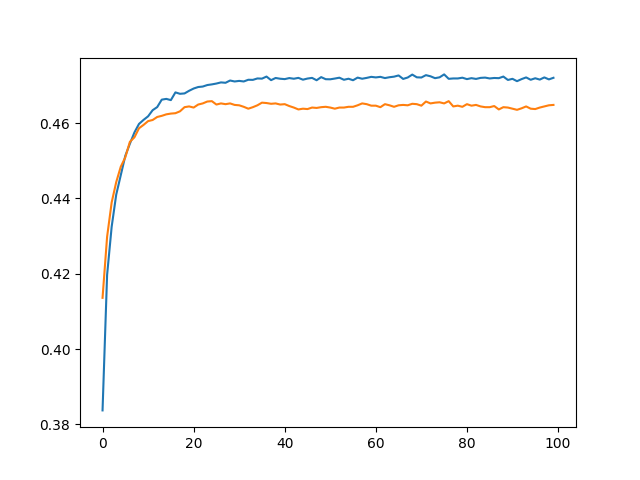
\includegraphics[scale=0.60]{hog_svm_accuracy}
  \caption{Validation Accuracy.}
  \label{fig:eg}
\end{figure}
\begin{figure}[h]
  \centering
  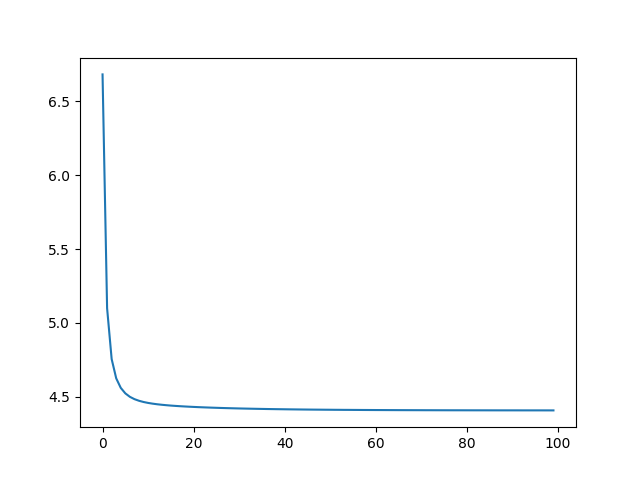
\includegraphics[scale=0.60]{hog_svm_loss}
  \caption{Validation Loss.}
  \label{fig:eg}
\end{figure}

\pagebreak

\subsection{Logistic Regression}
Best validation accuracy: 42.60\% \\
Test accuracy: 42.449\% \\
\begin{figure}[h]
  \centering
  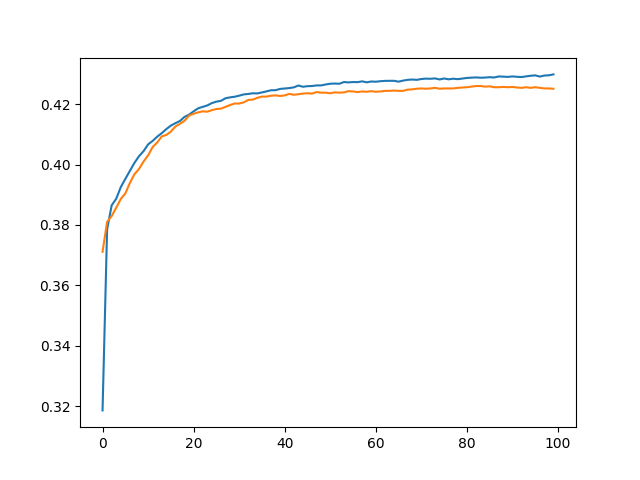
\includegraphics[scale=0.60]{hog_logreg_accuracy}
  \caption{Validation Accuracy.}
  \label{fig:eg}
\end{figure}
\begin{figure}[h]
  \centering
  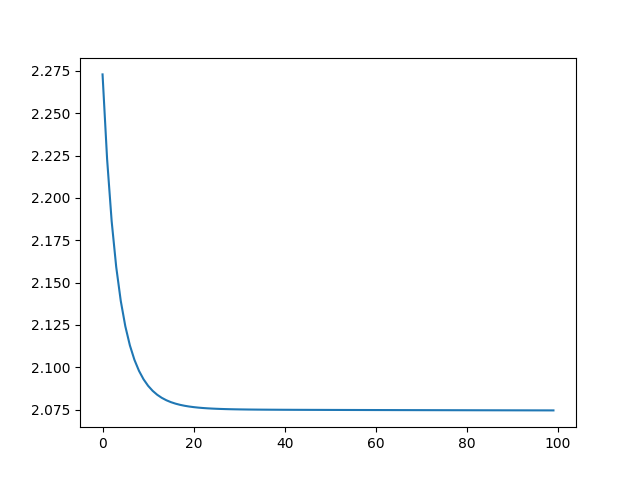
\includegraphics[scale=0.60]{hog_logreg_loss}
  \caption{Validation Loss.}
  \label{fig:eg}
\end{figure}

\pagebreak


\section{Cross validation results}
The following validation results were obtained by running the HOG model on
cifar-10 dataset with logistic regression and cross validation. Learning rate
was adjusted between tests, other parameters were left default.
\subsection{Learning Rate $10^-4$}
Average best validation accuracy: 42.95\% \\
Good learning rate because accuracy curve stabilizes at 43\% and loss curve
rapidly falls off and stabilizes.
\begin{figure}[h]
  \centering
  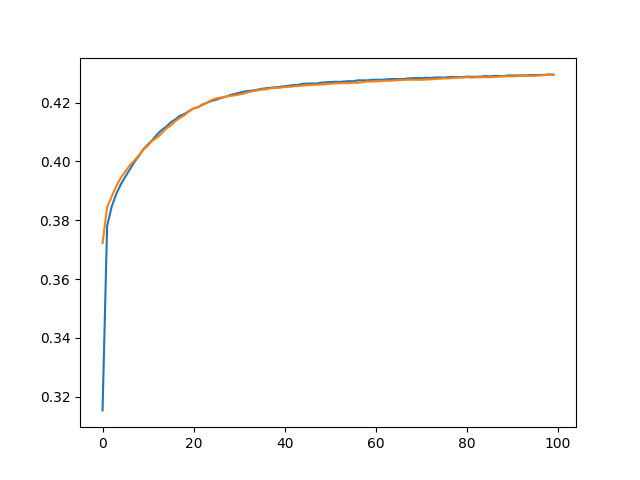
\includegraphics[scale=0.60]{hog_logreg_cv_lre4_acc}
  \caption{Validation Accuracy.}
  \label{fig:eg}
\end{figure}
\begin{figure}[h]
  \centering
  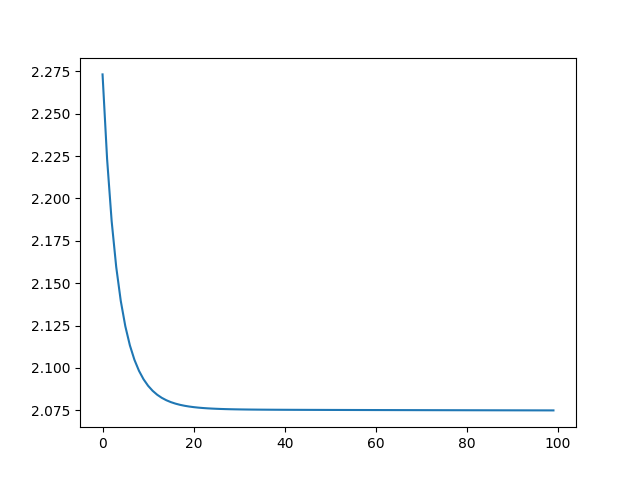
\includegraphics[scale=0.60]{hog_logreg_cv_lre4_loss}
  \caption{Validation Loss.}
  \label{fig:eg}
\end{figure}
\pagebreak

\subsection{Learning Rate $10^-2$}
Average best validation accuracy: 43.77\% \\
A bad learning rate because accuracy and loss curves never stabilize. This is
caused by the learning rate being too high, which causes the descent algorithm
to overshoot.
\begin{figure}[h]
  \centering
  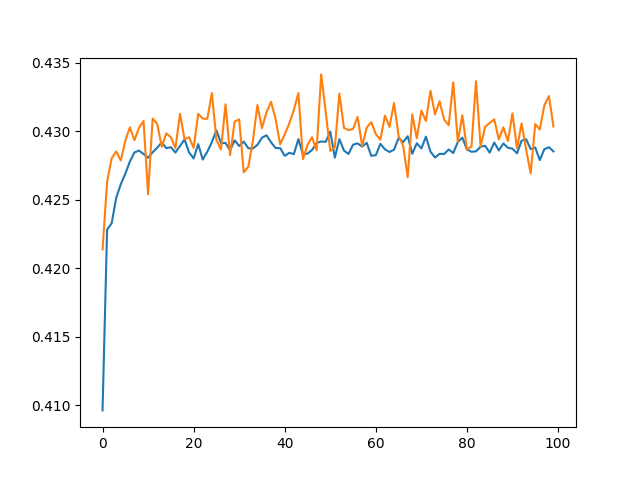
\includegraphics[scale=0.60]{hog_logreg_cv_lre2_acc}
  \caption{Validation Accuracy.}
  \label{fig:eg}
\end{figure}
\begin{figure}[h]
  \centering
  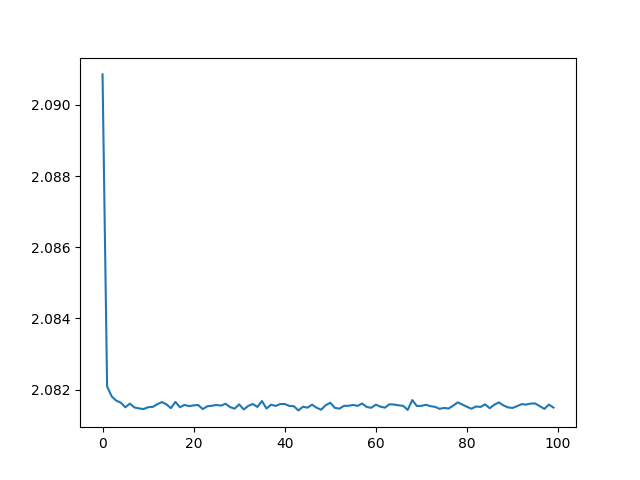
\includegraphics[scale=0.60]{hog_logreg_cv_lre2_loss}
  \caption{Validation Loss.}
  \label{fig:eg}
\end{figure}

\end{document}


%%% Local Variables:
%%% mode: latex
%%% TeX-master: t
%%% End:
